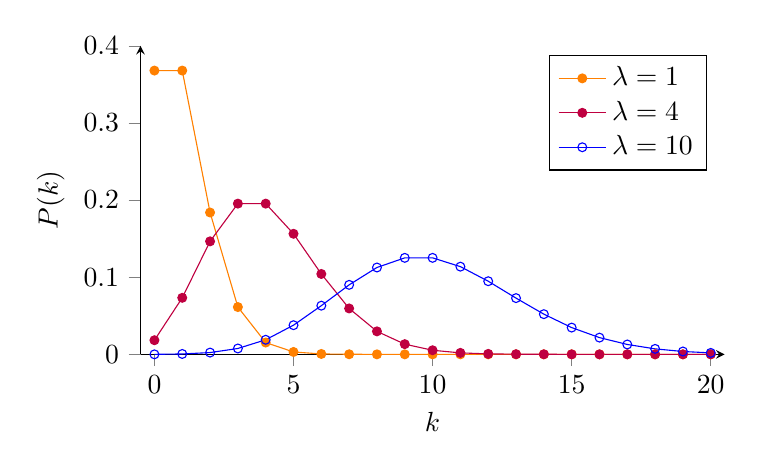
\begin{tikzpicture}
\begin{axis}[
  width=9cm, height=5.5cm,
  xlabel={$k$}, ylabel={$\mathbb{P}(k)$},
  xmin=-0.5, xmax=20.5, ymin=0, ymax=0.4,
  xtick={0,5,10,15,20},
  ytick={0,0.1,0.2,0.3,0.4},
  yticklabel style={/pgf/number format/fixed},
  legend pos=north east, legend cell align=left,
  axis lines=left, tick align=outside,
]
\addplot[orange, thin, mark=*, mark size=1.6pt] coordinates {(0,0.3679) (1,0.3679) (2,0.1839) (3,0.0613) (4,0.0153) (5,0.0031) (6,0.0005) (7,0.0001) (8,0.0000) (9,0.0000) (10,0.0000) (11,0.0000) (12,0.0000) (13,0.0000) (14,0.0000) (15,0.0000) (16,0.0000) (17,0.0000) (18,0.0000) (19,0.0000) (20,0.0000)};
\addlegendentry{$\lambda=1$}
\addplot[purple, thin, mark=*, mark size=1.6pt] coordinates {(0,0.0183) (1,0.0733) (2,0.1465) (3,0.1954) (4,0.1954) (5,0.1563) (6,0.1042) (7,0.0595) (8,0.0298) (9,0.0132) (10,0.0053) (11,0.0019) (12,0.0006) (13,0.0002) (14,0.0001) (15,0.0000) (16,0.0000) (17,0.0000) (18,0.0000) (19,0.0000) (20,0.0000)};
\addlegendentry{$\lambda=4$}
\addplot[blue, thin, mark=o, mark size=1.6pt] coordinates {(0,0.0000) (1,0.0005) (2,0.0023) (3,0.0076) (4,0.0189) (5,0.0378) (6,0.0631) (7,0.0901) (8,0.1126) (9,0.1251) (10,0.1251) (11,0.1137) (12,0.0948) (13,0.0729) (14,0.0521) (15,0.0347) (16,0.0217) (17,0.0128) (18,0.0071) (19,0.0037) (20,0.0019)};
\addlegendentry{$\lambda=10$}
\end{axis}
\end{tikzpicture}
